The theses used for our analysis were taken from the ProQuest Full Text Thesis and Dissertation Database\footnote{Searchable via \texttt{http://search.proquest.com/pqdtft/}}. This database contains 1.5 million theses, when doing searches for English-language documents with full text available. The database includes metadata specifying features such as date of submission, University, Department, subject, and so on. All of this is freely available to licensed users -- notably, any user whose requests originates from within the IP block of a subscribing university (such as Princeton).

The data collection occurred in two stages: collecting the theses, and then running a parsing and extraction routine on them to pull out the text of the acknowledgements section.  Figure~\ref{fig:data_collect_block_diagram} shows a block diagram of this data collection process.

\begin{figure}
	\centering
	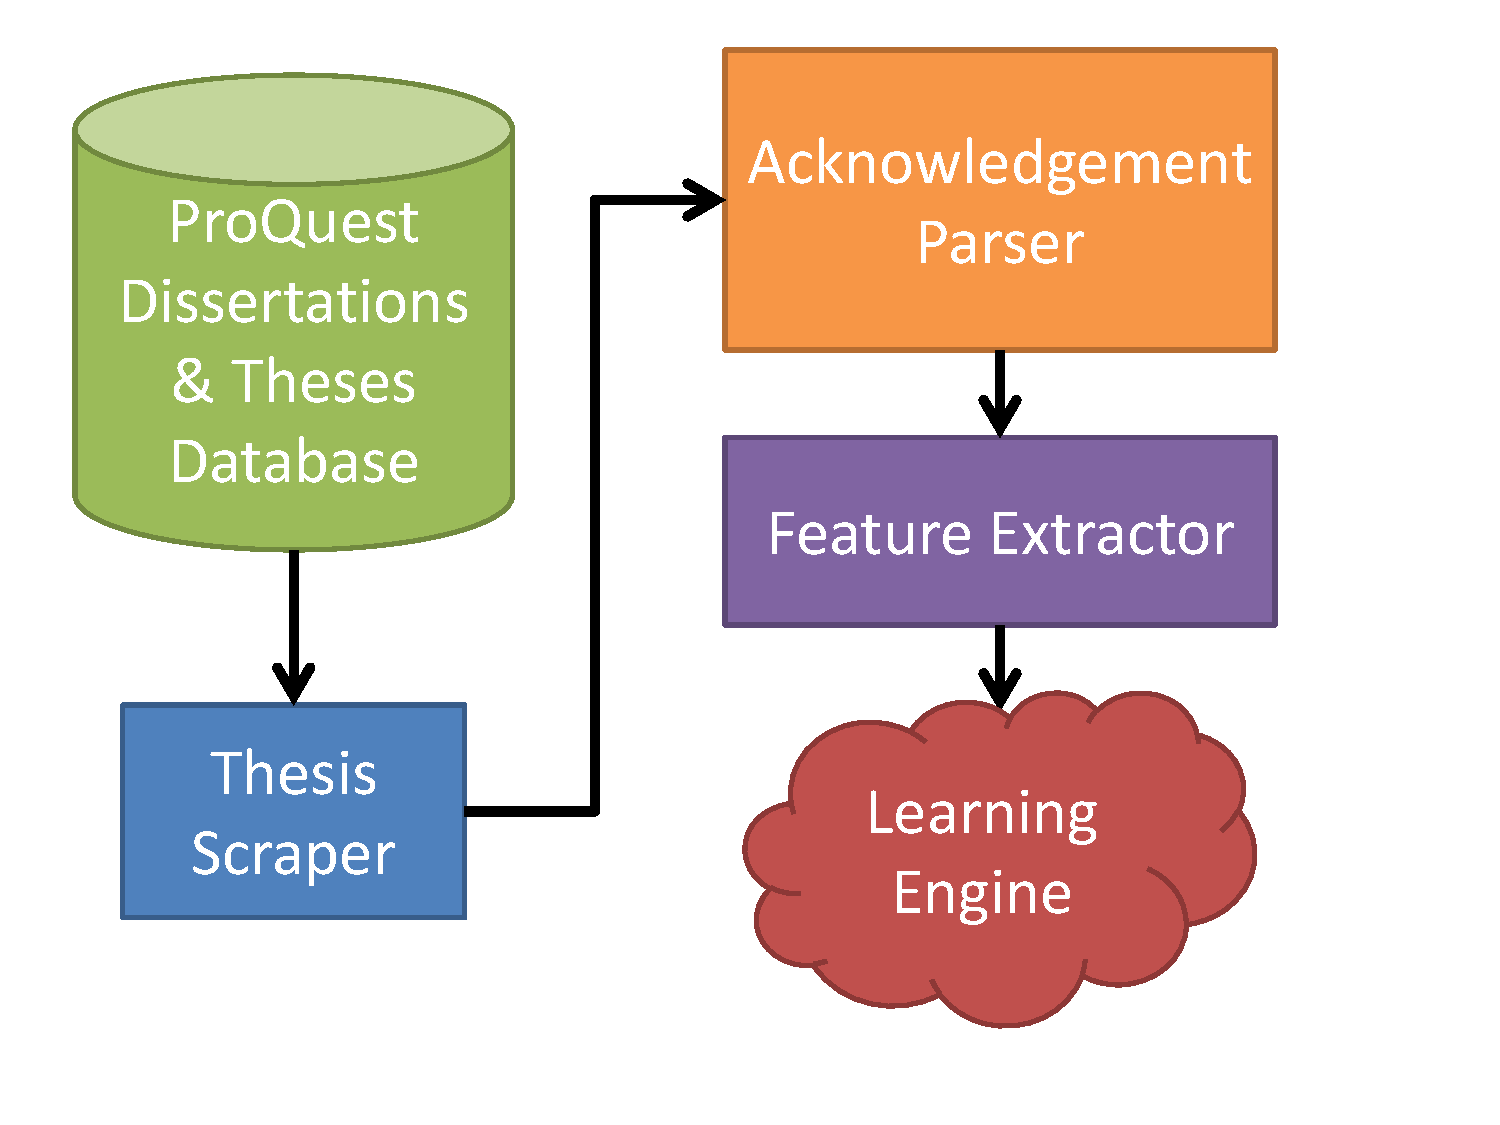
\includegraphics[width=0.7\textwidth]{block_diagram}
	\caption{Block diagram showing the data collection process}
	\label{fig:data_collect_block_diagram}
\end{figure}

\subsection*{Collecting theses (scraping)}
ProQuest has a database API exposed at \texttt{http://fedsearch.proquest.com/}. This access point seems to accept SRU (Search/Retrieval via URL)\footnote{See \texttt{http://www.loc.gov/standards/sru/}} queries, but fails to respond to the standard \texttt{Explain} operation, thus making its valid query terms unaccessible. Documentation for the service appears to be non-existent.\footnote{Though one user reports the existence of a document available from ProQuest on request: see \texttt{bibwild.wordpress.com/a-proquest-platform-api/}. He claims it is not very explanatory.}

We were successful in reverse-engineering the API to the extent where we could collect 1000 URLs of fulltext English theses. This is the dataset we went on to use for an analysis of PhD satisfaction by state over the United States. However, this dataset was insufficient for any analysis of individual universities.

At this point we switched to scraping documents via the standard, human-facing ProQuest search interface. When queries are made through this interface, ProQuest attempts to authenticate the humanity of the downloader using captcha-gateways for any downloads beyond a small number. Via various subterfuges, however, we were able to circumvent these measures and download 200 theses for each of the Ivy League universities.\footnote{The number 200 was chosen mainly to keep data processing times reasonable. With enough time (or compute power), our method should be easily extensible to at least several thousand theses per university} These form our second dataset.

Throughout this stage of the collection process we made extensive use of the Python packages \texttt{requests} and \texttt{BeautifulSoup} for HTTP requests and HTML parsing respectively.

\subsection*{Feature Extraction}

After scraping the PDFs and metadata for each thesis, the next task, as shown in Figure~\ref{fig:data_collect_block_diagram}, was to parse out the acknowledgement section.  This proved to be a more challenging task than we originally thought, thus, we had to resort to ad-hoc methods for identifying the location of the acknowledgement section within the PDF.

We extract the text from the PDF using \texttt{pdftotext}, which comes standard with the Xpdf\footnote{http://www.foolabs.com/xpdf/download.html} package in most linux installations.  This was the most robust solution we found in comparison with some Python PDF parsing libraries.  The output from \texttt{pdftotext} is a text file with the extracted text from the PDF.  The next task was to identify the acknowledgement section and parse it out.

Identifying the acknowledgement sections boiled down to identifying headings in the PDF.  Headings always occured on their own line and were relatively short.  When analyzing the text for headings, all page breaks, numbers, and punctuation were removed.  In addition, all the characters were converted to lower-case and all whitespace was removed.  This left headings on a single line and removed variation in capitalization, numbering of sections, etc.  

After identifying headings, it was trivial to find the start of the acknowledgements section, just look for the word acknowledgements (in practice I had to use some variations of acknowledgement, as there were some typos in this heading as well as spelling difference, such as "acknowledgment" versus "acknowledgement").  The removing of whitespace and other distracting characters avoided the case of identifying the acknowledgements listing in the table of contents as the actual acknowledgement section for most cases.  However, for some cases, we had to check that the acknowledgement heading and the terminating heading did not occur on the same page, as this would indicate we most likely found the table of contents.  The more difficult part was finding where the acknowledgement section ended.  Here we had to resort to going through many PDFs and finding common sections that follow the acknowledgement section.  This included "Table of Contents, "Abstract", "Dedication", "Introduction", etc.  Then we simply looked for these headings to identify where the acknowledgement section ended.  This allowed us to parse the large majority of acknowledgement sections, although we may miss a few that use non-standard headings or sections following the acknowledgement sections.

There were a couple caveats to parsing the acknowledgement section.  First, if the thesis had no acknowledgements section, the text returned would be empty.  This is exactly what we want, as we still wanted to include theses without acknowledgements in our data since the fact the student didn't write an acknowledgement section may say something about their satisfaction.  Second, if we found the acknowledgements section heading, but did not find a terminating heading after 5 pages of the PDF, we gave up and dropped that thesis from our data set.  This case indicates that we most likely missed the terminating heading (did not include it in our set of headings following the acknowledgement sections), since acknowledgement sections are generally less than 5 pages.  

The next step, as shown in Figure~\ref{fig:data_collect_block_diagram}, is to extract features from the acknowledgement section text.  This step was rather trivial.  We first converted all the characters to lower case, removed line and page breaks, removed digits, removed punctuation, and removed some odd UTF-8 characters that were parsed out of the PDF.  We then split all the words by whitespace, leaving us with an array of words in Python.  We used the Python Natural Language Toolkit\footnote{http://www.nltk.org/} (nltk) to remove stopwords and perform stemming.  We then converted this to a bag of words, i.e. list of counts for each word occuring in the document.  We returned the bag of words and total word count for analysis.